\documentclass[aspectratio=169,t,11pt,table]{beamer}
\usepackage{../includes/slides,../includes/math}
\definecolor{accent}{HTML}{2B5269}
\definecolor{accent2}{HTML}{9D2235}

\title{Introduction to Forecasting}
\subtitle{\it  ECON 5753 — University of Arkansas}
\date{Sprint 2025}
\author{Prof. Kyle Butts}


\begin{document}

% ------------------------------------------------------------------------------
\begin{frame}[noframenumbering,plain]
\maketitle
\end{frame}
% ------------------------------------------------------------------------------


% ------------------------------------------------------------------------------
\section{Forecasting}
% ------------------------------------------------------------------------------

\begin{frame}{Problem of Prediction}
  The goal of forecasting is to learn the relationship between \alert{input variables} and \alert{outcome variable(s)} so that we can \alert{predict} the outcome variables when we do not observe it. 

  \pause
  \bigskip
  E.g., Learn about who are potential customers to advertise to based on their observable characteristics
  \begin{itemize}
    \item Input: observable characteristics
    \item Outcome: whether they purchase a product
  \end{itemize}
    
  \pause
  \bigskip
  Predict values of a variable in the future, e.g. \alert{time-series} of stock prices
  \begin{itemize}
    \item Input: the time-period
    \item Output: stock price
  \end{itemize}
\end{frame}

\begin{frame}{Model}
  We have an outcome variable $y$ and a set of $p$ different predictor variables $X = (X_1, X_2, \dots, X_p)$. 
  \begin{itemize}
    \item For some observations we observe both $X$ and $Y$
    \begin{itemize}
      \item Essential to \alert{\emph{fit}} the model, i.e. learn the relationship between the two
    \end{itemize}
  \end{itemize}

  \bigskip
  We can write the model in a general form as
  $$
    y = f_0(X) + \varepsilon,
  $$
  where $f_0$ is some unknown function of $X$ and $\varepsilon$ is the \alert{error term}.
\end{frame}

\begin{frame}{Model}
  \vspace*{-\bigskipamount}
  $$
    y = f_0(X) + \varepsilon,
  $$

  Here we think of $f_0(X)$ as the `true' model: this is the best prediction of $y$ given information on $X$. In this case we assume $\expec{y - f_0(X)}{X} = \expec{\varepsilon}{X} = 0$
  \begin{itemize}
    \item Once we know $f_0(X)$, we can not predict any more of the variation in $y$ using $X$
  \end{itemize}
\end{frame}

\begin{frame}{Prediction of $f$}
  We will use a training sample of data to predict $f_0$. We will denote our estimate of $f_0$ as $\hat{f}$. For a given unit, we predict 
  $$
    \hat{y} = \hat{f}(X)
  $$
\end{frame}

\begin{frame}{Error term}
  The term `error term' is a bit overloaded. It's worth trying to clarify:

  \bigskip
  \begin{enumerate}
    \item If we knew the `true' model, $f_0(X)$, then $\varepsilon \equiv y - f_0(X)$ represents the things that are unpredictable given $X$
    \begin{itemize}
      \item This is the ``true'' error term
    \end{itemize}

    \bigskip
    \item If $\hat{f}(X)$ is an estimated model, $\hat{\varepsilon} = y - \hat{f}(X)$ is the difference between that unit's $y_i$ and their predicted $y$, $f(X_i)$
    \begin{itemize}
      \item This is better called the \alert{prediction error}
    \end{itemize}
  \end{enumerate}
\end{frame}

\begin{frame}{Error term}
  \begin{center}
    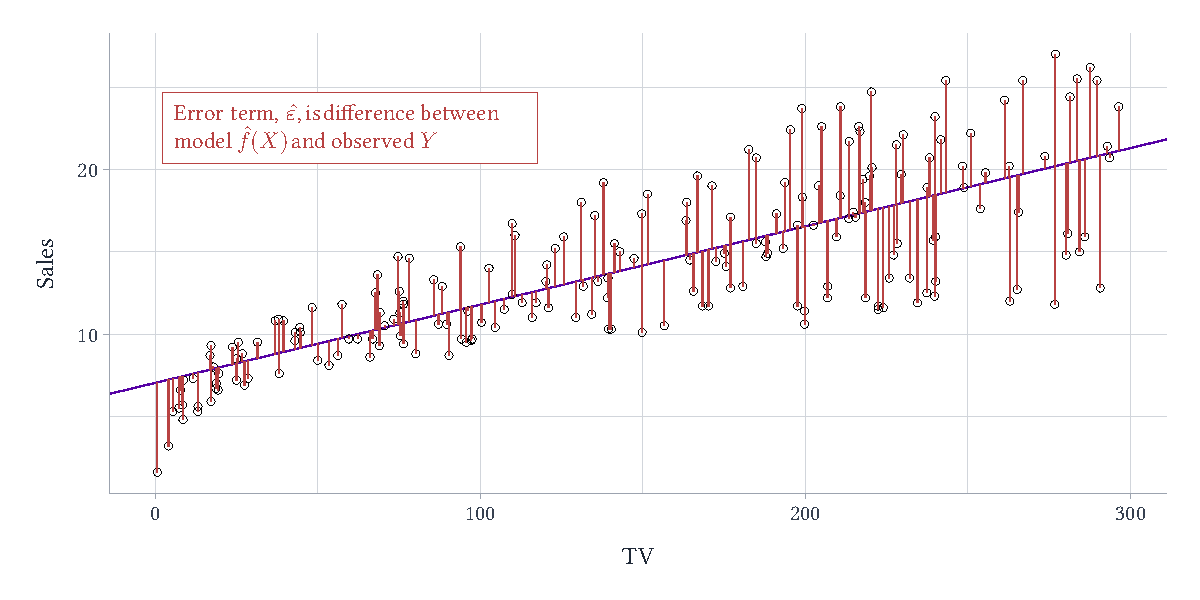
\includegraphics[width=0.9\textwidth]{figures/sales_tv_error_term.pdf}
  \end{center}
\end{frame}

% ------------------------------------------------------------------------------
\section{Goals of Forecasting}
% ------------------------------------------------------------------------------

\begin{frame}{Goals of estimation of $f$}
  There are two related goals when predicting $f$:
  \begin{enumerate}
    \item Predict $y$ as well as possible (\alert{prediction})
    \begin{itemize}
      \item Think of prediction as a `black box' where the goal is to do as good of a job at predicting $y$ as possible
      
      \item Want to learn the `true' $f_0(X)$, leaving no information on the table
    \end{itemize}
    
    \bigskip
    \item Understand the relationship between $X$ and $y$ (\alert{inference})
    \begin{itemize}
      \item If our goal is being able to describe the relationship between $x$ and $y$; i.e. we care about understanding $f_0$ and not just $\hat{y}$
      
      \item Worth approximating $f_0$ with a more `simple' functional form so that we can better convey the results to stakeholders. 
      \begin{itemize}
        \item Creates ``heuristics'' that helps decision-makers
      \end{itemize}
    \end{itemize}
  \end{enumerate}
\end{frame}

\begin{frame}{Examples of Prediction vs. Inference}
  Say we are thinking about housing:
  \begin{itemize}
    \item Example of prediction: ``Is the house over/under-priced''
    \begin{itemize}
      \item Only care about $\hat{\text{price}} = f(X)$
    \end{itemize}

    \bigskip
    \item Example of inference: ``How much more do homes with a river view sell for?''
    \begin{itemize}
      \item Need to know information about $f$ to answer
    \end{itemize}
  \end{itemize}
\end{frame}

\imageframe{figures/f_examples_plot_raw.pdf}
\imageframe{figures/f_examples_plot_pred_1.pdf}
\imageframe{figures/f_examples_plot_pred_2.pdf}
\imageframe{figures/f_examples_plot_pred_3.pdf}
\imageframe{figures/f_examples_plot_pred_4.pdf}

\begin{frame}{Model Flexibility}
  There is a limit to how \alert{flexible} we can make our model
 
  \bigskip
  \begin{enumerate}
    \item If our goal is prediciton, we only have a finite amount of data to use to fit the model, so there's a limit on how much we can learn
    \begin{itemize}
      \item Face the risk of \alert{overfitting} the data (chasing after the random noise $\varepsilon$)
    \end{itemize}
   
    \bigskip
    \item If our goal is inference, then added flexibility is harder to summarize to stakeholders.
  \end{enumerate}
\end{frame}

\imageframe{figures/f_examples_plot_pred_4.pdf}

\section{Fitting Models}

\begin{frame}{High-level of fitting models}
  The general framework for forecasting is as follows:
  \begin{enumerate}
    \item Collect a set of data $\{ (y_i, X_i) \}_{i=1}^n$ for a set of observations.
    
    \bigskip
    \item Using knowledge of the topic, select a \alert{class} of models $\mathcal{F}$ that you want to select from
    \begin{itemize}
      \item That is, $\hat{f}$ must be one of the functions in $\mathcal{F}$, e.g. linear functions of $X_i$
    \end{itemize}
    
    \bigskip
    \item Using your data, select $\hat{f} \in \mathcal{F}$ that \emph{predicts} $y$ ``best''
    \begin{itemize}
      \item ``best'' is defined by a \alert{loss function}, e.g. mean-squared prediction error
    \end{itemize}
  \end{enumerate}
\end{frame}

\begin{frame}{Selecting class of models}
  Let's break this down. First, we have to select a class of models $\mathcal{F}$
  \begin{itemize}
    \item This involves selecting variables we want to include in the model
    
    \item Specifying a functional form for the model
  \end{itemize}

  \pause
  \bigskip
  For example, we might think about a simple \emph{linear model} of our $X$ variables:
  $$
    f(X_i) = \alpha + X_{i1} \beta_1 + X_{i2} \beta_2
  $$
  
  $\mathcal{F}$ would consist of all the models of this form, i.e. we are selecting over values of $(\alpha, \beta_1, \beta_2)$
\end{frame}

\begin{frame}{title}
  For example, we might think about a simple \emph{linear model} of our $X$ variables:
  $$
    f(X_i) = \alpha + X_{i1} \beta_1 + X_{i2} \beta_2
  $$


  This is a restrictive model:
  \begin{itemize}
    \item no polynomials of $X_1$ (e.g. wages are non-linear in age)
    \item no interaction between $X_1$ and $X_2$ (e.g. college degree changes return to experience)
  \end{itemize} 
\end{frame}

\begin{frame}{Selecting class of models}
  Perhaps, we want to look within a wider class of $\mathcal{F}$:
  $$
    f(X_i) = \alpha + X_{i1} \beta_1 + X_{i1}^2 \beta_2 + X_{i2} \beta_3 + X_{i2}^2 \beta_4 + X_{i1} X_{i2} \beta_5 + u_i
  $$
 
  \bigskip
  $\mathcal{F}$ consists of all functions of this form
  \begin{itemize}
    \item some of the coefficients can be 0, so this class is \emph{strictly} more general than the last.
  \end{itemize}
  
  \pause
  \bigskip
  Can imagine creating a bunch more terms or having things other than quadratics
  \begin{itemize}
    \item e.g. $\one{20 < \text{Age}_i \leq 30}$
  \end{itemize} 
\end{frame}

\begin{frame}{Prediction Error}
  We want to be able to evaluate which model in our selected class, $\mathcal{F}$, does the ``best'' job at predicting $y$. 
  
  \bigskip
  Given a model $f \in \mathcal{F}$, we want to evaluate how good our model does at predicting observations $y$. For this, define the \alert{prediction error} as 
  $$
    \hat{\varepsilon} = \underbrace{y}_{\text{true value}} - \underbrace{f(X)}_{\text{predicted value}}
  $$

  \begin{itemize}
    \item[$\rightarrow$] The prediction error depends on the choice of model $f \in \mathcal{F}$
  \end{itemize}
\end{frame}

\begin{frame}{Prediction Error}
  $$
    \hat{\varepsilon} = \underbrace{y}_{\text{true value}} - \underbrace{f(X)}_{\text{predicted value}}
  $$

  \bigskip
  Large $\hat{\varepsilon}$ means you did a poor job of predicting that observation. That could be because of
  \begin{enumerate}
    \item \alert{Reducible errors}: The model is bad at predicting $y$, i.e. $f(X) \neq f_0(X)$
    
    \item \alert{Irreducible errors}: Or, the true noise $\varepsilon$ is making $y$ far away from the systematic component $f(X)$ for this observation
  \end{enumerate}
\end{frame}

\begin{frame}{Prediction Error}
  We can rewrite our prediction error as
  \begin{align*}
    \hat{\varepsilon} &= y - f(X) \\
    &= f_0(X) + \varepsilon - f(X) \\
    &= \underbrace{f_0(X) - f(X)}_{\text{reducible}} + \underbrace{\varepsilon}_{\text{irreducible}}
  \end{align*}

  \bigskip
  {\color{blue} Remember:} we do not know $f_0$, so we can not separate the two.
\end{frame}

\begin{frame}{Loss functions}
  To provide a summary measure of fit, we want to \emph{average} prediction error over many observations. This will find a `average' prediction error

  \bigskip
  If we took the simple mean of prediction error, positive and negative prediction errors would cancel out
  \begin{itemize}
    \item An error of -1 and 1 would be just as bad as -4 and 4.
  \end{itemize}
\end{frame}

\begin{frame}{Loss functions: Mean-squared prediction error}
  The most common loss-function is the \alert{mean-square (prediction) error} (MSE):
  \begin{equation}\label{eq:mspe}
    \text{MSE} \equiv \frac{1}{n} \sum_{i=1}^n \left( y_i - \hat{y}_i \right)^2 = \frac{1}{n} \sum_{i=1}^n \hat{\varepsilon}_i^2
  \end{equation}

  \bigskip
  \pause
  If we collect $\hat{\varepsilon}_i$ as a vector, we can use linear algebra to more simply write it as 
  $$
    \text{MSE} = \frac{1}{n} \hat{\varepsilon}' \hat{\varepsilon}
  $$
\end{frame}

\begin{frame}{Mean-square prediction error}
  \begin{columns}[T]
    \begin{column}{.3\textwidth}\vspace*{-\bigskipamount}
      \begin{table}[H]
\centering
\begin{tblr}[         %% tabularray outer open
]                     %% tabularray outer close
{                     %% tabularray inner open
colspec={Q[]Q[]Q[]},
row{even}={bg=black!5!white},
colsep = {1em},
}                     %% tabularray inner close
\toprule
$y_i$ & $\hat{y}_i$ & $\hat{\varepsilon}_i$ \\ \midrule %% TinyTableHeader
3.7 & 4.20 & \only<2>{0.5} \\
4.1 & 4.18 & \only<2>{0.08} \\
5.6 & 5.48 & \only<2>{-0.12} \\
2.9 & 3.29 & \only<2>{0.39} \\
8.8 & 8.81 & \only<2>{0.01} \\
\bottomrule
\end{tblr}
\end{table}

    \end{column}
    \hfill
    \begin{column}{.6\textwidth}
      Calculate mean-square prediction error:

      \only<2>{\begin{align*}
  \text{MSPE} &= \frac{1}{5} \left( 0.5^2 + 0.08^2 + -0.12^2 + 0.39^2 + 0.01^2 \right) \\
  &= 0.0846
\end{align*}}
    \end{column}
  \end{columns}
\end{frame}

\begin{frame}{Loss functions}
  The mean-squared prediction error is not the only loss-function:
  \begin{itemize}
    \item The mean-absolute prediction error $\frac{1}{n} \sum_{i=1}^n \left\vert y_i - \hat{y}_i \right\vert$ 
    \begin{itemize}
      \item Will estimate the \emph{median} of $y$ given $X$
    \end{itemize}
    
    \pause
    \item Imagine a setting where you're predicting whether someone has a disease; you would want to penalize false-negatives more than false-positives
  \end{itemize}
\end{frame}

\begin{frame}{In-sample vs. Out-of-sample prediction error}
  As a forecaster, you will \alert{fit} a model using a set of observations $\left\{ (x_1, y_1), \dots, (x_n, y_n) \right\}$. This is called the \alert{training data}.

  \bigskip
  We can calculate the \alert{in-sample MSE} by formula (\ref{eq:mspe}) averaging over all observations in the training data.
  \begin{itemize}
    \item This tells us how good we do at predicting the data \emph{we trained the model on}.
  \end{itemize} 
\end{frame}  

\begin{frame}{In-sample vs. Out-of-sample prediction error}
  If our goal is prediction, we really want to know how the model would predict on \emph{new} observations that we \emph{have not seen before}
  \begin{itemize}
    \item It is common to hold out a set of \alert{test data} that is NOT used for training the model, but just for evaluating it's performance
  \end{itemize}
\end{frame}

\begin{frame}{Why use `test data'?}
  It is common to try and `pick' from a set of models based on how they do at in-sample prediction:
  \begin{itemize}
    \item That is, select the model with the smallest \emph{in-sample MSE}. 
  \end{itemize}

  \pause
  \bigskip
  This is \emph{a bad thing to do}; by focusing on fitting the current sample very well, you are risking \alert{overfitting} the data
\end{frame}

\begin{frame}{Flexibility vs. Overfitting}
  \vspace{-\bigskipamount}
  \begin{center}
    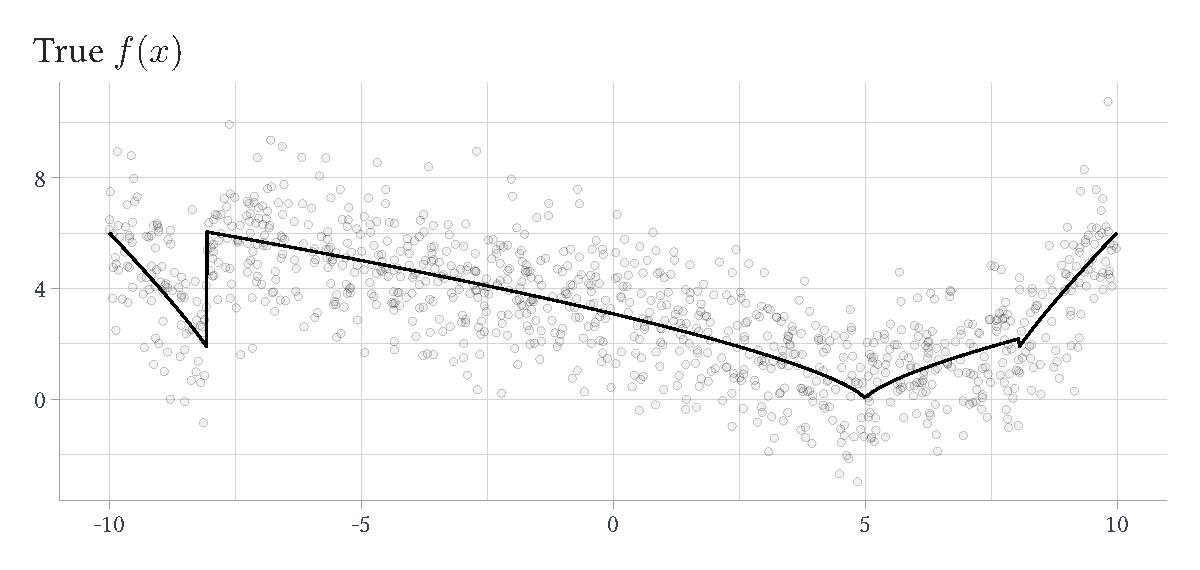
\includegraphics[width = \textwidth]{figures/f_examples_plot_dgp.pdf}
  \end{center}
\end{frame}

\begin{frame}{Flexibility vs. Overfitting}
  \vspace{-\bigskipamount}
  \begin{center}
    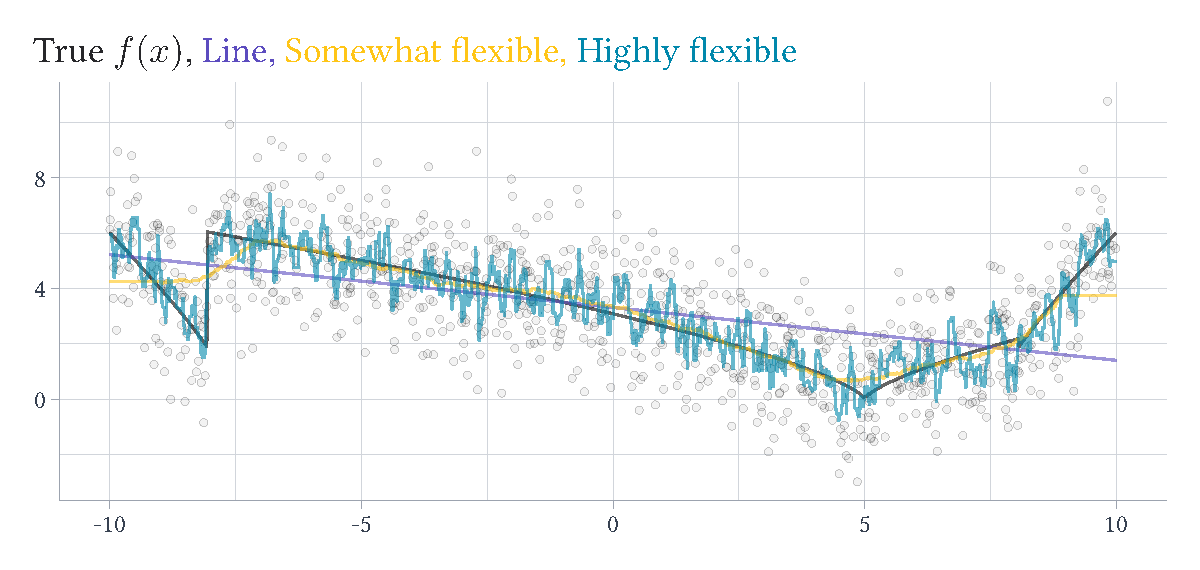
\includegraphics[width = \textwidth]{figures/f_examples_overfitting.pdf}
  \end{center}
\end{frame}

\begin{frame}{Flexibility vs. Overfitting}
  By making the model more and more \emph{flexible}, you risk overfitting more and more

  \begin{itemize}
    \item Your model tries to improve the \emph{in-sample} mean-squared error, but it worstens your \emph{out-of-sample} MSE.
  \end{itemize}
  
  \bigskip
  A solution is to evaluate your model fit using outside `testing data'
\end{frame}

\begin{frame}{Sample-splitting}
  We will not spend much time in this course discussing sample-splitting/cross-validation and model selection, but I want to give just one example so you're aware of it
  \begin{itemize}
    \item A lot of you might recognize this from Hyunseok's class
  \end{itemize}

  \pause
  \bigskip
  Say you want to fit a polynomial, but are concerned with over-fitting.
  We can tackle this with sample-splitting:
  \begin{itemize}
    \item Take a random half your data and fit a polynomial of order $k$
    \item Evaluate MSE on the other half your data (test set)
  \end{itemize}
  
  \bigskip
  Do this for $k = 1, \dots, K$ and pick the polynomial degree that minimizes test-data MSE
  \begin{itemize}
    \item See ILSR section 5.1 for cross-validation 
  \end{itemize}
\end{frame}

\begin{frame}{Sample-splitting}  
  This technique is not as common when your model is more simple (e.g. regression model with a few terms)
  \begin{itemize}
    \item In some sense, you are preventing yourself from overfitting by making the model simple
  \end{itemize}
\end{frame}

\begin{frame}{High-level of fitting models}
  The general framework for forecasting is as follows:
  \begin{enumerate}
    \item Collect a set of data $(y, X)$ for a set of observations.
    
    \item Using knowledge of the topic, select a \alert{class} of models $\mathcal{F}$ that you want to select from
    \begin{itemize}
      \item That is, $\hat{f}$ must be one of the functions in $\mathcal{F}$.
    \end{itemize}
    
    \item Using your data (\emph{perhaps on a training sample}), select $\hat{f} \in \mathcal{F}$ that minimizes the \alert{loss function}
    \begin{itemize}
      \item E.g. mean-squared prediction error (\emph{perhaps on testing sample})
    \end{itemize}
  \end{enumerate}
\end{frame}

\begin{frame}{Bias-variance trade-off}
  This discussion of increasing flexiblity leading to increasing the noise of the model fit is a well-known problem. It is called the \alert{Bias-Variance Tradeoff}:
  \begin{enumerate}
    \item \alert{Bias}: When the model we fit, $\hat{f}(x)$, does a poor job fitting the true model $f_0(x)$
    
    \item \alert{Variance}: The variability of the model we fit, $\hat{f}(x)$, across samples
    \begin{itemize}
      \item Repeated sampling: the model we estimate varies from estimate to estimate
    \end{itemize}
  \end{enumerate}

  \pause
  \bigskip
  This is a `trade-off'. To lower bias by adding flexibility, you're adding variance (noisiness) to the estimate 
\end{frame}

\subsection{Model Selection: Adveristing Example}

\begin{frame}{Model Selection}
  Our general approach seems to follow:
  \begin{itemize}
    \item Select class of models to choose from, $\mathcal{F}$.
    
    \item Find $\hat{f} \in \mathcal{F}$ that minimizes the in- or out-of- sample MSPE
  \end{itemize}
  
  \bigskip
  The secret sauce of forecasting is in selecting $\mathcal{F}$
  \begin{itemize}
    \item E.g. sports teams all have a ton of data to help them draft the best players; all will minimize MSPE to fit their model; all will do sample-splitting; etc. 
    \begin{itemize}
      \item The advantage is who can pick the best \alert{variables} to include in their model
      \item Often called ``\alert{feature selection}''
    \end{itemize}
  \end{itemize} 
\end{frame}

\begin{frame}{Model Selection: Advertising Example}
  Say you're a business and you want to use advertising to boost sales. You have a bunch of different markets (e.g. cities) and you have data on how you've spent your advertising budget in those markets and the sales in that market
\end{frame}

\begin{frame}{Advertising Example}{Single-variable predictors}
  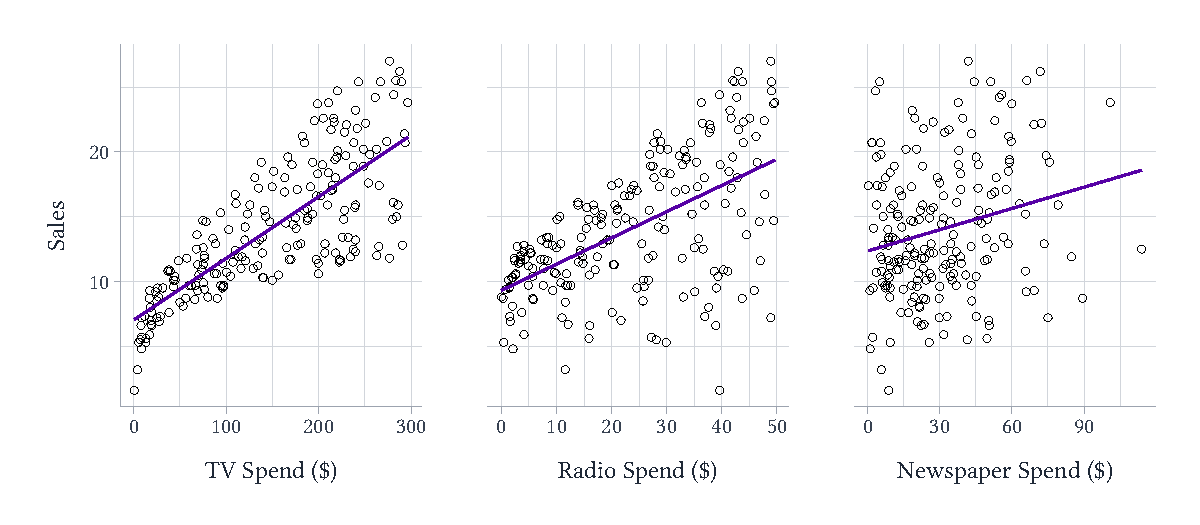
\includegraphics[width=\textwidth]{figures/sales_bivariate.pdf}
\end{frame}

\begin{frame}{Advertising Example}
  We see that sales are higher in markets that have spending on TV, Radio, and Newspaper ads separately. 
  
  \pause
  \bigskip 
  These single scatter plots with line of best-fits are a somewhat poor model:
  \begin{itemize}
    \item Are there synergies between different advertising strategies (are they substitutes or complements to one another)?

    \item Do places with more TV ads also have more radio ads? Then how can we tell if it is TV ads that are helping or if it is really radio ads 
  \end{itemize}

  \pause\bigskip
  \alert{Key takeaway:} Forecasting models get better the more carefully you think about the context you are in
\end{frame}

\begin{frame}{Interactions Matter}
  Over the next few weeks, we will learn a lot about regression methodology. We will do so for a set of covariates, $X_i$. 
  \begin{itemize}
    \item These could be a set of variables like age, height, batting average, etc.
    \item But, these could also be functions of variables, e.g. $\one{\text{Age}_i = 21}$ or height $\times$ weight
  \end{itemize}

  \bigskip
  It is important to remember that the world can feature a lot of non-linearities and interactive effects
  \begin{itemize}
    \item Your model should reflect those too! 
  \end{itemize}
\end{frame}


\section{Sample Distribution}

\begin{frame}{Estimands vs. Estimators}
  % \bgPurple{Parameters} come from models of how observed data are generated, e.g. $y = f_0(X) + u_i$
  % \begin{itemize}
  %   \item The target for an empirical analysis: what we want to know
  % \end{itemize}\pause
  % 
  % \bigskip
  \textbf{\rose{Estimands}} are functions of the population data distribution. 
  What you would estimate if you observed \emph{everyone} in your population of interest
  \begin{itemize}
    \item E.g. a population mean or population line of best fit
  \end{itemize}\pause
  
  \bigskip
  \textbf{\blue{Estimators}} are functions of the observed data itself (the ``sample'')
  \begin{itemize}
    \item E.g. a sample mean or OLS coefficients
  \end{itemize}

  \bigskip
  Since your sample is random, so is your estimator. Each estimator has a distribution that we will call the \emph{sample distribution}
\end{frame}
  
\begin{frame}{The Lay of the Land}
  \bigskip
  \begin{adjustbox}{width = 0.75\textwidth, center}
    % Tikz settings optimized for causal graphs.
    \tikzset{
        -Latex,auto, node distance =1 cm and 1 cm, semithick,
        state/.style ={ellipse, draw, minimum width = 0.7 cm},
        point/.style = {circle, draw, inner sep=0.04cm,fill,node contents={}},
        bidirected/.style={Latex-Latex,dashed},
        el/.style = {inner sep=2pt, align=left, sloped}
    }
    \begin{tikzpicture}
      % \node[purple] (theory) at (-4, 1.25) {Economic Theory};
      % \node[state,rectangle,purple] (parameters) at (-4, 0) {Parameters};
      
      \node[rose] (distribution) at (-2.5, 1.25) {Population Distribution};
      \node[state,rectangle,rose] (estimands) at (-2.5, 0) {Estimands};

      \node[blue] (data) at (2.5, 1.25) {Observed Sample};
      \node[state,rectangle,blue] (estimators) at (2.5, 0) {Estimators};

      % \path[purple, thick, shorten >=4pt] (theory) edge (parameters);
      \path[rose, thick, shorten >=4pt] (distribution) edge (estimands);
      \path[blue, thick, shorten >=4pt] (data) edge (estimators);

      % \path[thick, shorten >=4pt, shorten <=4pt] (estimands) edge[bend left= 40] node[below, el, yshift=-4pt] {Identification} (parameters);
      \path[thick, shorten >=4pt, shorten <=4pt] (estimators) edge[bend left= 40] node[below, el, yshift=-4pt] {Statistical Inference} (estimands);
    \end{tikzpicture}
  \end{adjustbox}
\end{frame}
  
\begin{frame}{Population Regression}
  The OLS \blue{\emph{estimator} $\hat{\beta}_{\text{OLS}}$} consistently estimates the regression \rose{\emph{estimand} $\beta_{\text{OLS}}$} under relatively weak conditions


  \bigskip
  Our statistical software uses a sample to estimate $\blue{\hat{\beta}_{\text{OLS}}}$ and with our estimate we \emph{infer} about $\rose{\beta_{\text{OLS}}}$. With inference, we can say: 
  
  \smallskip
  \begin{enumerate}
    \item Our best guess at $\rose{\beta_{\text{OLS}}}$ is $\blue{\hat{\beta}_{\text{OLS}}}$
    
    \smallskip
    \item With 95\% confidence, $\rose{\beta_{\text{OLS}}}$ falls within the range 
    $$
    [\blue{\hat{\beta}_{\text{OLS}}} - 1.96 * SE(\hat{\beta}_{\text{OLS}}), \blue{\hat{\beta}_{\text{OLS}}} + 1.96 * SE(\hat{\beta}_{\text{OLS}})]
    $$
  \end{enumerate}
\end{frame}

\begin{frame}{Repeated Sampling}
  When doing forecasting, we will observe \emph{a single random sample} from the population. But, for conducting inference about the population parameter, it is useful to use the \alert{repeated sampling} perspective:
  \begin{itemize}
    \item Imagine drawing a bunch of random samples of the sample size from the population. Let $b$ denote each random sample.
    
    \item For each sample, form that sample's estimate $\hat{\theta}_b$
  \end{itemize}

  \pause
  \bigskip
  Since each sample is different, you have a distribution of $\hat{\theta}_b$. This is called the \alert{sampling distribution} of the estimator.
\end{frame}

\begin{frame}{Sample Distribution}
  \begin{columns}[T]
    \begin{column}{.33\textwidth}
    \end{column}
    \hfill
    \begin{column}{.67\textwidth}
      \vspace*{-\bigskipamount}
      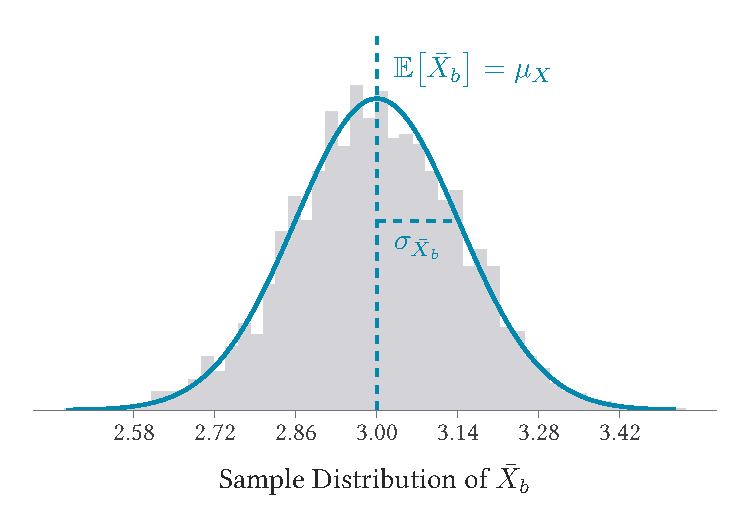
\includegraphics[width = \textwidth]{figures/sample_dist.pdf}
    \end{column}
  \end{columns}
  \begin{tikzpicture}[remember picture, overlay]
    \begin{scope}[shift={(3,3.8)}] 
      \node[anchor = east] at (0, 1) {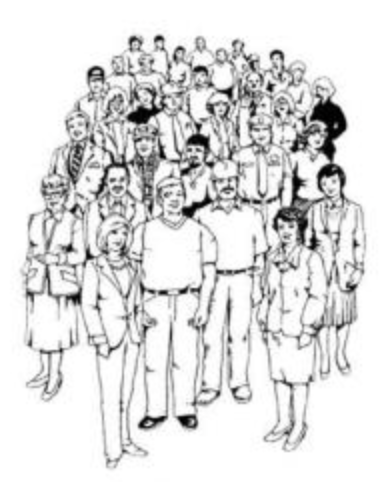
\includegraphics[width = 0.2\textwidth]{figures/pop.png}};
      \node[anchor = north, align = center] at (-1.5, -0.7) {\small Population mean};
      \node[anchor = north, align = center] at (-1.5, -1.2) {\small $\mu = 3$};

      % SRS size 10 lines
      \draw[thick] (0,1.8) -- (2.5,1.8) node[pos=1,right] {$\bar{X}_1 = 2.92$};
      \node[anchor = south, align = center] at (1.2,1.8) {\footnotesize sample of size $n$};

      \draw[thick] (0,0.8) -- (2.5,0.8) node[pos=1,right] {$\bar{X}_2 = 3.18$};
      \node[anchor = south, align = center] at (1.2,0.8) {\footnotesize sample of size $n$};

      \draw[thick] (0,-0.2) -- (2.5,-0.2) node[pos=1,right] {$\bar{X}_3 = 3.02$};
      \node[anchor = south, align = center] at (1.2,-0.2) {\footnotesize sample of size $n$};
      
      \node[anchor = north] at (3.3, -0.7) {$\vdots$};
      
      \draw[decorate, decoration = {brace, amplitude = 7pt}] (4.5, 2) -- (4.5,-0.4);
    \end{scope}
  \end{tikzpicture}
\end{frame}

\begin{frame}{Sample Distribution}
  The remarkable thing about sample distributions is that \emph{most of the time} our estimators have a sample distribution that is a \emph{normal distribution}. This is due to the \alert{central limit theorem}
\end{frame}

\begin{frame}{Unbiased Estimators}
  An estimator is \alert{unbiased} if $\expec{\hat{\theta}_b} = \theta$, the estimator is on average (across repeated samples) equal to the estimand
\end{frame}

\begin{frame}{Consistent Estimators}
  An estimator is \alert{consistent} if as $n \to \infty$
  \begin{enumerate}
    \item $\expec{\hat{\theta}_b} \to \theta$ and
    \item the standard deviation of the sample distribution of $\hat{\theta}_b$ collapse to $0$
  \end{enumerate} 

  \bigskip
  If you have a large enough sample, your sample estimator approaches the estimand
\end{frame}



\section{Types of Data}

\begin{frame}{Cross-sectional Data}
  
  \begin{columns}[T]
    \begin{column}{.4\textwidth}
      \alert{Cross-sectional data} consists of many different \emph{units} viewed at a point in time:
    \end{column}
    \begin{column}{.6\textwidth}
      \vspace*{-\bigskipamount}
      \begin{table}[H]
\centering
\begin{tblr}[         %% tabularray outer open
]                     %% tabularray outer close
{                     %% tabularray inner open
colspec={Q[]Q[]Q[]Q[]},
row{even}={bg=black!5!white},
colsep = {1em},
}                     %% tabularray inner close
\toprule
school\_id & avg\_sat\_math & pct\_white & pct\_black \\ \midrule %% TinyTableHeader
01M539 & 657 & 28.6\% & 13.3\% \\
02M294 & 395 & 11.7\% & 38.5\% \\
02M308 & 418 & 3.1\% & 28.2\% \\
02M545 & 613 & 1.7\% & 3.1\% \\
01M292 & 410 & 3.9\% & 24.4\% \\
01M696 & 634 & 45.3\% & 17.2\% \\
\bottomrule
\end{tblr}
\end{table}

    \end{column}
  \end{columns}
\end{frame}

\begin{frame}{Time-series Data}
  \begin{columns}[T]
    \begin{column}{.4\textwidth}
      \alert{Time-series data} consists of a single observational unit viewed over multiple points in time:
    \end{column}
    \begin{column}{.6\textwidth}
      \vspace*{-\bigskipamount}
      \begin{table}[H]
\centering
\begin{tblr}[         %% tabularray outer open
]                     %% tabularray outer close
{                     %% tabularray inner open
colspec={Q[]Q[]Q[]Q[]Q[]},
row{even}={bg=black!5!white},
colsep = {1em},
}                     %% tabularray inner close
\toprule
month & day & hour & bikers & temp \\ \midrule %% TinyTableHeader
1 &  1 & 0  & 16 & 0.24 \\
1 &  1 & 1  & 40 & 0.22 \\
1 &  1 & 2  & 32 & 0.22 \\
$\vdots$ & $\vdots$ & $\vdots$ & $\vdots$ & $\vdots$ \\
12 & 31 & 21 & 52 & 0.40 \\
12 & 31 & 22 & 38 & 0.38 \\
12 & 31 & 23 & 31 & 0.36 \\
\bottomrule
\end{tblr}
\end{table}

    \end{column}
  \end{columns}
\end{frame}

\begin{frame}{Panel Data}
  \begin{columns}[T]
    \begin{column}{.4\textwidth}
      \alert{Panel data} is like time-series data, but for many different observational units:
    \end{column}
    \begin{column}{.6\textwidth}
      \vspace*{-\bigskipamount}
      \begin{table}[H]
\centering
\begin{tblr}[         %% tabularray outer open
]                     %% tabularray outer close
{                     %% tabularray inner open
colspec={Q[]Q[]Q[]},
row{even}={bg=black!5!white},
colsep = {1em},
}                     %% tabularray inner close
\toprule
fund\_manager & month & return \\ \midrule %% TinyTableHeader
1 &  1 & -3.34\% \\
1 &  2 & 3.76\% \\
1 &  3 & 12.97\% \\
$\vdots$ & $\vdots$ & $\vdots$ \\
2000 & 48 & -3.76\% \\
2000 & 49 & 2.25\% \\
2000 & 50 & 6.68\% \\
\bottomrule
\end{tblr}
\end{table}

    \end{column}
  \end{columns}
\end{frame}



\end{document}
